\documentclass{article}
\usepackage[utf8]{inputenc}
\usepackage[T1]{fontenc}
\usepackage[ngerman]{babel}
\usepackage{fancyhdr}
\usepackage{geometry}
\usepackage[table]{xcolor}
\usepackage{amsmath}
\usepackage{amssymb}
\usepackage{tabularx}
\usepackage{multicol}
\usepackage{listings}
\usepackage{graphicx}
\usepackage{wrapfig}

\geometry{
    a4paper,
    top=30mm,
    bottom=30mm,
    left=20mm,
    right=20mm,
}

\newcommand*{\qed}{\hfill\ensuremath{\square}}

\setlength{\parskip}{1em}
\setlength{\parindent}{0em}

\pagestyle{fancy}
\fancyhf{}
\lhead{AaS-Benchmark}
\rhead{Alexander Korn}
\rfoot{\thepage}

\begin{document}

\begin{center}
    \large \textbf{Übersicht über die Funktionalität von AaS-Benchmark mit Beispielen}
\end{center}

\vspace{2em}

\begin{multicols*}{2}
    {\setlength{\parskip}{0em} \tableofcontents}

    \section{Einleitung}

    \textit{AaS-Benchmark} ist ein Tool, das es ermöglicht, die Ausführungszeiten von Algorithmen aus der Vorlesung \textit{Algorithmen auf Sequenzen} zu messen. Dabei können verschiedenste Parameter gewählt werden, um so beispielsweise Zusammenhänge von Musterlängen und Ausführungszeiten zu erkennen. Die Algorithmen aus der Vorlesung sowie dieses Tool wurden dazu in der Programmiersprache \textit{Rust} implementiert.
    
    In dieser Übersicht sollen dem Leser die verschiedenen Funktionen von AaS-Benchmark nähergebracht und mit einigen Beispielen demonstriert werden.

    \section{Algorithmen}

    Für Aas-Benchmark wurden elf Algorithmen aus der Vorlesung implementiert. Diese lassen sich wie folgt in drei Kategorien aufteilen:

    \subsection{Algorithmen für einzelne Muster}

    Diese Gruppe von Algorithmen findet alle Vorkommen eines einzelnen Musters in einem Text. Implementiert sind in dieser Gruppe die folgenden Algorithmen:

    \begin{itemize}
        \setlength{\parskip}{0em}
        \item Naiver Algorithmus
        \item Knuth-Morris-Pratt
        \item Shift-And
        \item BNDM
    \end{itemize}

    \subsection{Algorithmen für mehrere Muster}

    Diese Gruppe enthält Algorithmen, die alle Vorkommen von Mustern aus einer gegebenen Menge in einem Text finden. Sie unterscheiden sich also insofern von den Algorithmen der letzten Gruppe, als dass sie nicht mit nur nach einem einzelnen Muster suchen, sondern nach mehreren Mustern gleichzeitig.

    Hier sind ein naiver Algorithmus, sowie der Aho-Corasick Algorithmus implementiert.

    \subsection{Fehlertolerante Algorithmen}

    \subsection{Volltextindizes}

    \section{Das Ausgabeformat}

    Wurde Aas-Benchmark korrekt ausgeführt, erhält man eine Ausgabe, die der Form der in Listing \ref{lst:output_format_example} gezeigten Daten entspricht. Diese Ausgabe hat das CSV Format, es handelt sich also um eine Tabelle, bei der die Spalten je Zeile durch Kommata getrennt sind. Die erste Zeile enthält dabei den Tabellenkopf.

    Jede Zeile steht für eine einzelne Ausführung des Algorithmus, der in der ersten Spalte der Zeile gegeben ist. Die Spalten enthalten die folgenden Informationen:

    \begin{itemize}
        \setlength{\parskip}{0em}
        \item \texttt{algorithm}: Der ausgeführte Algorithmus
        \item \texttt{text\_length}: Die Länge des Textes bei dieser Ausführung
        \item \texttt{pattern\_length}: Die Länge des Musters bei dieser Ausführung
        \item \texttt{execution}: Die wievielte Ausführung dies ist
        \item \texttt{matches}: Wie viele Vorkommen des Musters bei dieser Ausführung im Text gefunden wurden
        \item \texttt{prep\_time\_ms}: Die benötigte Vorbereitungszeit in Millisekunden\footnote{Bei Algorithmen, die keine Vorbereitungszeit benötigen immer 0}
        \item \texttt{time\_ms}: Die benötigte Zeit, um den Algorithmus mit den gegebenen Parametern auszuführen
    \end{itemize}

    \section{Nutzung}

    \subsection{Wahl der Algorithmen}

    \subsection{Mehrere Ausführungen}

    \subsection{Textquellen}

    \newpage

    \section{Beispiele}

    Beginnen wir mit einem einfachen Beispiel. Wir möchten testen, wie sich die Laufzeit des naiven Algorithmus für die Mustersuche bei steigender Musterlänge verhält.

    Der Befehl für die Ausführung von AaS-Benchmark könnte dafür zum Beispiel wie folgt aussehen:

    \texttt{./aas-benchmark naive -t 100000000 -p 1..10}

    \begin{wrapfigure}{l}{0.65\linewidth}
        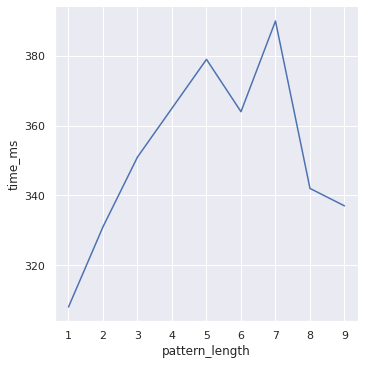
\includegraphics[width=\linewidth]{assets/graph_1.png}
        \caption{Laufzeit des naiven Algorithmus}
    \end{wrapfigure}

    Lässt man sich die Ausgabe dieses Befehls plotten, so erhält man das Diagramm in Abbildung 1. So kann man mit Aas-Benchmark das Verhalten der implementierten Algorithmen einfach betrachten und die verschiedenen Algorithmen miteinander vergleichen.

    Als nächsten schauen wir uns ein einfaches Beispiel an, bei dem die Laufzeit zweier Algorithmen bei steigender Musterlänge geprüft wurde. Dazu wurde der folgende Befehl verwendet:

    \texttt{./aas-benchmark kmp,horspool -t 100000000 -p 1..10}

    \begin{wrapfigure}{r}{0.65\linewidth}
        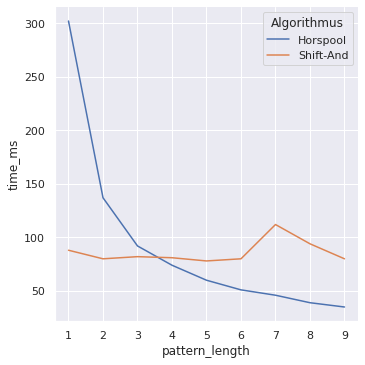
\includegraphics[width=\linewidth]{assets/graph_2.png}
        \caption{Laufzeit des naiven Algorithmus}
    \end{wrapfigure}

    Lässt man sich die Aufgabe erneut plotten, kann man nun erkennen, dass der \textit{Horspool} Algorithmus mit steigender Musterlänge immer schneller ausgeführt werden kann, während die Laufzeit des \textit{Shift-And} Algorithmus relativ konstant bleibt.

\end{multicols*}

\lstinputlisting[caption=Beispiel des Ausgabeformates, captionpos=b, frame=single, label=lst:output_format_example]{assets/output_format_example.csv}

\begin{multicols*}{2}
    test
\end{multicols*}

\end{document}
